\documentclass[spanish,letterpaper,oneside]{article}

\def\documenttitle {Balance de fertilización N-P-K}
\def\documentsubtitle {Producto Integrador de Aprendizaje: sistemas lineales en agronomía}
\def\documentsubject {PIA - Álgebra Lineal}
\def\documentauthor {Equipo de Álgebra Lineal}
\def\coursename {Álgebra Lineal}
\def\coursecode {PIA}
\def\universityname {Universidad Autónoma de Nuevo León}
\def\universityfaculty {Facultad de Agronomía}
\def\universitydepartment {Ingeniero Agrónomo}
\def\universitydepartmentimage {UANL/assets-uanl/logo-uanl.png}
\def\universitydepartmentimagecfg {width=2.1cm}
\def\universitylocation {General Escobedo, Nuevo León, México}
\def\authortable {
  \begin{tabular}{llll}
    \textbf{Integrante} & \textbf{Nombre completo} & \textbf{Matrícula} & \textbf{Grupo} \\
    1 & Por completar & Por completar & Por completar \\
    2 & Por completar & Por completar & Por completar \\
    3 & Por completar & Por completar & Por completar \\
    4 & Por completar & Por completar & Por completar \\
    \multicolumn{4}{l}{Programa: Ingeniero Agrónomo} \\
    \multicolumn{4}{l}{Semestre: agosto--diciembre de 2026} \\
    \multicolumn{4}{l}{Fecha límite: 11 de noviembre de 2026} \\
    \multicolumn{4}{l}{\universitylocation}
  \end{tabular}
}

\AddToHook{file/config.tex/after}{\def\stylecitereferences{custom}}
\AddToHook{file/config.tex/after}[aulatex-algebra-lineal]{%
  \def\documentfontsize{12}
  \def\documentinterline{1}
  \def\documentparindent{0}
  \def\documentparskip{5}
  \def\fontdocument{custom}
  \def\fonttypewriter{custom}
  \def\stylecitereferences{custom}
  \def\portraitstyle{style1}
  \def\hfstyle{style1}
  \def\hfwidthwrap{true}
  \def\hfwidthtitle{0.44}
  \def\hfwidthcourse{0.52}
  \def\predocpageromannumber{false}
  \def\pagemarginleft{2.5}
  \def\pagemarginright{2.5}
  \def\pagemargintop{2.5}
  \def\pagemarginbottom{2.5}
  \def\firstpagemargintop{3.8}
  \def\sectionfontsize{\large}
  \def\sectionspacingtop{8}
  \def\sectionspacingbottom{4}
  \def\ssectionfontsize{\normalsize}
  \def\ssectionspacingtop{6}
  \def\ssectionspacingbottom{3}
  \def\defaultimagefolder{UANL/img/}
  \def\usepdfmetadata{false}
}
% Template:     Informe LaTeX
% Documento:    Núcleo del template
% Versión:      DEV
% Codificación: UTF-8
%
% Autor: Pablo Pizarro R.
%        pablo@ppizarror.com
%
% Manual template: [https://latex.ppizarror.com/informe]
% Licencia MIT:    [https://opensource.org/licenses/MIT]

% -----------------------------------------------------------------------------
% CONFIGURACIONES
% -----------------------------------------------------------------------------
% Definiciones previas
\input{src/defs}

% Ajustes usuario
\input{src/config}

% -----------------------------------------------------------------------------
% IMPORTACIÓN DE LIBRERÍAS
% -----------------------------------------------------------------------------
\input{src/env/imports}

% -----------------------------------------------------------------------------
% IMPORTACIÓN DE FUNCIONES Y ENTORNOS
% -----------------------------------------------------------------------------
\input{src/cmd/core}
\input{src/cmd/math}
\input{src/cmd/equation}
\input{src/cmd/image}
\input{src/cmd/title}
\input{src/cmd/other}
\input{src/cmd/column}
\input{src/env/environments}

% -----------------------------------------------------------------------------
% IMPORTACIÓN DE ESTILOS
% -----------------------------------------------------------------------------
\input{src/style/code}
\input{src/style/other}

% -----------------------------------------------------------------------------
% CONFIGURACIÓN INICIAL DEL DOCUMENTO
% -----------------------------------------------------------------------------
\input{src/cfg/init}

% -----------------------------------------------------------------------------
% PORTADA
% -----------------------------------------------------------------------------
\input{src/page/portrait}
\input{src/page/portrait_config}

% -----------------------------------------------------------------------------
% CONFIGURACIÓN DE PÁGINA Y ENCABEZADOS
% -----------------------------------------------------------------------------
\input{src/cfg/page}

% -----------------------------------------------------------------------------
% TABLA DE CONTENIDOS - ÍNDICE
% -----------------------------------------------------------------------------
\input{src/page/index}

% -----------------------------------------------------------------------------
% CONFIGURACIONES FINALES
% -----------------------------------------------------------------------------
\input{src/cfg/final}

\RemoveFromHook{file/config.tex/after}[aulatex-algebra-lineal]


\usepackage[backend=biber,style=apa,natbib=true]{biblatex}
\addbibresource{UANL/ingeniero-agronomo/algebra-lineal/algebra-lineal.bib}
\usepackage{pgfplots}
\usetikzlibrary{babel}
\pgfplotsset{compat=1.18}
\definecolor{piagreen}{RGB}{39,105,74}
\definecolor{piablue}{RGB}{42,102,153}
\definecolor{piagold}{RGB}{184,133,33}
\pdfcompresslevel=9
\pdfobjcompresslevel=3

\begin{document}
\templatePortrait
\templatePagecfg
\onehalfspacing

\begin{abstractd}
Un balance de fertilización para un escenario didáctico de maíz relaciona tres
fórmulas N-P-K con metas de 99 kg/ha de N, 83 kg/ha de P$_2$O$_5$ y 84 kg/ha de
K$_2$O. La eliminación de Gauss-Jordan produce una solución única de 200, 300
y 100 kg/ha, respectivamente, verificada mediante determinantes y sustitución.
El resultado satisface el balance de nutrientes declarado, pero no demuestra
optimalidad económica, absorción efectiva por el cultivo ni idoneidad de una
recomendación de campo. Estas últimas requieren datos agronómicos adicionales.
\end{abstractd}

\templateIndex
\templateFinalcfg

\section{Introducción}
\subsection{Justificación}
Un sistema lineal representa relaciones simultáneas entre cantidades desconocidas.
En un problema de mezclas, cada coeficiente expresa la contribución de un insumo
a una meta; resolver el sistema permite determinar si las cantidades elegidas
satisfacen todas las condiciones a la vez \citep{strang2023introduction}.
En agronomía, esta estructura resulta útil para comprobar balances de fertilización
y detectar incompatibilidades entre las composiciones y las metas propuestas.

El análisis garantizado de un fertilizante expresa porcentajes en masa en el
orden N, P$_2$O$_5$ y K$_2$O. La elección de una dosis debe apoyarse en el análisis
del suelo y las necesidades de las plantas, no únicamente en una solución
numérica \citep{umn2024fertilizing}. Las cantidades de P$_2$O$_5$ y K$_2$O son
equivalentes de declaración: no deben confundirse con masas de fósforo y potasio
elementales ni con la cantidad que el cultivo absorberá.

\subsection{Planteamiento del problema}
Se considera un escenario didáctico de producción de maíz en Nuevo León.
Se fijan metas de aporte por hectárea de 99 kg de N, 83 kg de P$_2$O$_5$ y 84 kg
de K$_2$O y tres composiciones nominales: A, 12-24-12; B, 20-10-10; y C, 15-05-30.
Las metas y las fórmulas son supuestos del ejercicio; no representan un diagnóstico
de suelo documentado ni fichas verificadas de marcas comerciales.

La pregunta es: ¿qué cantidad de cada fórmula permite alcanzar simultáneamente
las tres metas con cantidades no negativas? Se busca un balance exacto; no se
plantea minimizar costos ni maximizar rendimiento.

\section{Recolección de datos}
La revisión documental permite establecer cómo interpretar el grado N-P-K y
por qué una aplicación real requiere conocer suelo, cultivo y condiciones de
manejo \citep{umn2024fertilizing}. Para el cálculo se adoptan los datos de la
tabla~\ref{tab:pia-datos}. Su naturaleza es didáctica: no se dispone de registros
de muestreo, resultados de laboratorio o etiquetas de productos que acrediten
las metas y composiciones específicas. Por ello, el caso no se presenta como
recolección experimental de datos de una unidad de producción.

\begin{table}[htbp]
\centering
\caption{Coeficientes nominales y metas del escenario didáctico.}
\label{tab:pia-datos}
\begin{tabular}{lrrrr}
\hline
Componente & A (kg/kg) & B (kg/kg) & C (kg/kg) & Meta (kg/ha) \\
\hline
N & 0.12 & 0.20 & 0.15 & 99 \\
P$_2$O$_5$ & 0.24 & 0.10 & 0.05 & 83 \\
K$_2$O & 0.12 & 0.10 & 0.30 & 84 \\
\hline
\end{tabular}
\end{table}

Cada coeficiente se obtiene dividiendo el porcentaje nominal entre 100. Así,
12\% de N equivale a 0.12 kg de N por kg de fórmula A. El producto de kg/kg
por kg/ha tiene unidades de kg/ha, iguales a las metas del balance.
La convención N-P-K se sustenta en la fuente universitaria; los valores elegidos
son parámetros del modelo, no dosis atribuidas a esa fuente.

\section{Metodología}
\subsection{Planteamiento del sistema}
Sean $x_1$, $x_2$ y $x_3$ las cantidades de las fórmulas A, B y C, respectivamente,
en kg/ha. Se supone composición constante, aditividad de aportes y ausencia de
pérdidas en el balance contable. No se modelan absorción, lixiviación ni
compatibilidad física de la mezcla. El sistema es
\begin{equation}
\begin{aligned}
0.12x_1+0.20x_2+0.15x_3 &= 99,\\
0.24x_1+0.10x_2+0.05x_3 &= 83,\\
0.12x_1+0.10x_2+0.30x_3 &= 84.
\end{aligned}
\label{eq:pia-sistema}
\end{equation}
Se añade la condición física $x_1,x_2,x_3\geq0$. Multiplicar cada ecuación
por 100 conserva sus soluciones y produce $A\mathbf{x}=\mathbf{b}$, donde
\[
A=\begin{pmatrix}12&20&15\\24&10&5\\12&10&30\end{pmatrix},\qquad
\mathbf{x}=\begin{pmatrix}x_1\\x_2\\x_3\end{pmatrix},\qquad
\mathbf{b}=\begin{pmatrix}9900\\8300\\8400\end{pmatrix}.
\]
La matriz decimal original es $A/100$; esta distinción evita confundir sus
determinantes al cambiar de escala.

\subsection{Justificación del método}
Se emplea Gauss-Jordan porque las operaciones elementales conservan el conjunto
de soluciones y permiten transformar la matriz aumentada en
$[I_3\mid\mathbf{x}]$. Los coeficientes 12, 24 y 12 facilitan la primera
eliminación. Se conserva aritmética exacta durante el procedimiento y se usa
la regla de Cramer como comprobación para una matriz cuadrada invertible
\citep{strang2023introduction}. Un determinante distinto de cero prueba
unicidad algebraica; la no negatividad debe comprobarse por separado.

\section{Procedimientos}
\subsection{Eliminación de Gauss-Jordan}
\textbf{Paso 1. Matriz inicial.}
\[
[A\mid\mathbf{b}]=\left[\begin{array}{rrr|r}
12&20&15&9900\\24&10&5&8300\\12&10&30&8400
\end{array}\right].
\]

\textbf{Paso 2. Eliminación bajo el primer pivote.}
Se aplican $R_2\leftarrow R_2-2R_1$ y $R_3\leftarrow R_3-R_1$:
\[
\left[\begin{array}{rrr|r}
12&20&15&9900\\0&-30&-25&-11500\\0&-10&15&-1500
\end{array}\right].
\]
En el segundo renglón, $8300-2(9900)=-11500$; en el tercero,
$8400-9900=-1500$.

\textbf{Paso 3. Segundo pivote.}
Se intercambian $R_2$ y $R_3$ y luego se divide el nuevo $R_2$ entre $-10$:
\[
\left[\begin{array}{rrr|r}
12&20&15&9900\\0&1&-3/2&150\\0&-30&-25&-11500
\end{array}\right].
\]

\textbf{Paso 4. Eliminación en la segunda columna.}
Con $R_1\leftarrow R_1-20R_2$ y $R_3\leftarrow R_3+30R_2$, se obtiene
\[
\left[\begin{array}{rrr|r}
12&0&45&6900\\0&1&-3/2&150\\0&0&-70&-7000
\end{array}\right].
\]
Los nuevos coeficientes de la tercera columna son
$15-20(-3/2)=45$ y $-25+30(-3/2)=-70$.

\textbf{Paso 5. Tercer pivote.}
La operación $R_3\leftarrow R_3/(-70)$ da
\[
\left[\begin{array}{rrr|r}
12&0&45&6900\\0&1&-3/2&150\\0&0&1&100
\end{array}\right].
\]

\textbf{Paso 6. Eliminación superior y normalización.}
Se aplican $R_2\leftarrow R_2+(3/2)R_3$ y $R_1\leftarrow R_1-45R_3$:
\[
\left[\begin{array}{rrr|r}
12&0&0&2400\\0&1&0&300\\0&0&1&100
\end{array}\right]
\xrightarrow{R_1\leftarrow R_1/12}
\left[\begin{array}{rrr|r}
1&0&0&200\\0&1&0&300\\0&0&1&100
\end{array}\right].
\]
Por tanto, $x_1=200$, $x_2=300$ y $x_3=100$ kg/ha.

\subsection{Regla de Cramer}
El determinante de la matriz entera se calcula por expansión de la primera fila:
\[
\Delta=12(300-50)-20(720-60)+15(240-120)=-8400\neq0.
\]
Para la matriz decimal, $\det(A/100)=\Delta/100^3=-0.0084$, también distinto
de cero. Al sustituir cada columna de $A$ por $\mathbf{b}$ se obtiene
\begin{align*}
\Delta_1&=\begin{vmatrix}9900&20&15\\8300&10&5\\8400&10&30\end{vmatrix}
=9900(250)-20(207000)+15(1000)=-1680000,\\
\Delta_2&=\begin{vmatrix}12&9900&15\\24&8300&5\\12&8400&30\end{vmatrix}
=12(207000)-9900(660)+15(102000)=-2520000,\\
\Delta_3&=\begin{vmatrix}12&20&9900\\24&10&8300\\12&10&8400\end{vmatrix}
=12(1000)-20(102000)+9900(120)=-840000.
\end{align*}
Los cocientes $x_1=\Delta_1/\Delta=200$, $x_2=\Delta_2/\Delta=300$ y
$x_3=\Delta_3/\Delta=100$ coinciden con Gauss-Jordan.

\subsection{Sustitución en el sistema original}
\begin{align*}
0.12(200)+0.20(300)+0.15(100)&=24+60+15=99,\\
0.24(200)+0.10(300)+0.05(100)&=48+30+5=83,\\
0.12(200)+0.10(300)+0.30(100)&=24+30+30=84.
\end{align*}
El residuo del sistema decimal es el vector cero. Las tres cantidades son
positivas, por lo que también satisfacen la restricción de no negatividad.

\subsection{Herramientas utilizadas}
El documento se elabora con LaTeX y la plantilla institucional AulaTeX; matrices,
sistemas y determinantes se componen como expresiones matemáticas nativas.
BibLaTeX con estilo APA y Biber gestionan las referencias; PGFPlots produce la figura vectorial a partir
de los aportes calculados. La compilación se realiza con TeX Live y latexmk.
Los determinantes y la sustitución se comprueban además mediante aritmética
independiente en PowerShell.

\section{Resultados}
La mezcla total del escenario es de 600 kg/ha. Si se supone una presentación
de 50 kg por bulto, las cantidades equivalen a 4, 6 y 2 bultos, respectivamente;
esa equivalencia no acredita una presentación comercial concreta.

\begin{table}[htbp]
\centering
\caption{Cantidades y aportes del balance calculado, en kg/ha.}
\label{tab:pia-resultados}
\begin{tabular}{lrrrr}
\hline
Fórmula & Cantidad & N & P$_2$O$_5$ & K$_2$O \\
\hline
A (12-24-12) & 200 & 24 & 48 & 24 \\
B (20-10-10) & 300 & 60 & 30 & 30 \\
C (15-05-30) & 100 & 15 & 5 & 30 \\
\hline
Total & 600 & 99 & 83 & 84 \\
\hline
\end{tabular}
\end{table}

\begin{figure}[htbp]
\centering
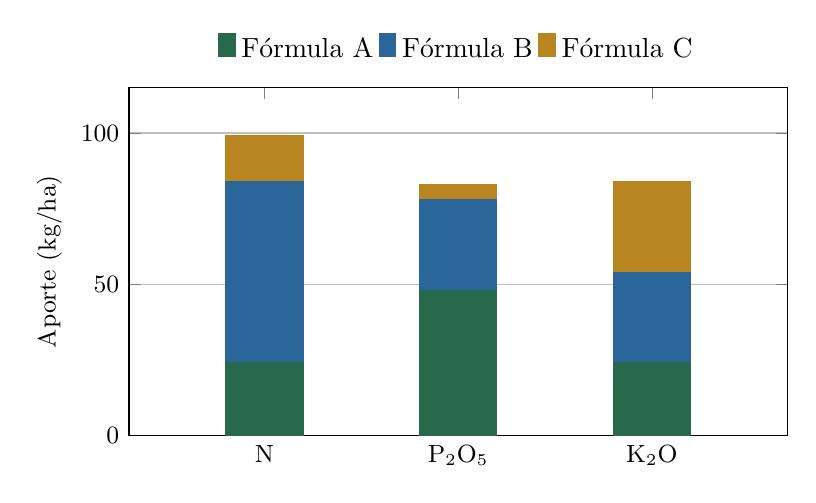
\begin{tikzpicture}
\begin{axis}[
  ybar stacked, bar width=28pt, width=0.82\linewidth, height=6cm,
  ymin=0, ymax=115, ylabel={Aporte (kg/ha)},
  symbolic x coords={N,P,K}, xtick=data,
  xticklabels={N,P$_2$O$_5$,K$_2$O},
  enlarge x limits=0.35, ymajorgrids=true,
  legend style={at={(0.5,1.04)},anchor=south,legend columns=3,draw=none},
  tick label style={font=\small}, label style={font=\small}]
\addplot[fill=piagreen,draw=piagreen] coordinates {(N,24) (P,48) (K,24)};
\addplot[fill=piablue,draw=piablue] coordinates {(N,60) (P,30) (K,30)};
\addplot[fill=piagold,draw=piagold] coordinates {(N,15) (P,5) (K,30)};
\legend{Fórmula A,Fórmula B,Fórmula C}
\end{axis}
\end{tikzpicture}
\caption{Aportes de las tres fórmulas: totales de 99, 83 y 84 kg/ha.
Elaboración a partir de los parámetros del escenario didáctico.}
\label{fig:pia-balance}
\end{figure}

\section{Análisis de resultados}
La fórmula B aporta $60/99\times100\approx60.6\%$ del N total; A aporta
$48/83\times100\approx57.8\%$ del P$_2$O$_5$; B y C aportan cada una
$30/84\times100\approx35.7\%$ del K$_2$O. Estos porcentajes describen el
origen del aporte, no la eficiencia de absorción del cultivo.

La solución es única porque $\det(A)\neq0$. Esto no implica que sea una mezcla
óptima: no se incluyen precios, presupuesto, rendimiento ni una función
objetivo. Tampoco la positividad demuestra compatibilidad física de productos,
ausencia de pérdidas o seguridad de una aplicación. Tales decisiones requieren
etiquetas, diagnóstico del suelo y evaluación técnica del cultivo
\citep{umn2024fertilizing}.

El fraccionamiento temporal debe respetar el acoplamiento de los nutrientes.
Por ejemplo, aplicar primero 200 kg de A, 50 kg de B y 100 kg de C aportaría
$(49,58,59)$ kg/ha de N, P$_2$O$_5$ y K$_2$O. Los 250 kg restantes de B
aportarían $(50,25,25)$ kg/ha. La suma conserva el balance total, pero la primera
aplicación no contiene todo el fósforo ni todo el potasio. Este ejemplo es una
comprobación aritmética, no una recomendación de calendario.

De hecho, como las tres fórmulas aportan cantidades positivas de P$_2$O$_5$ y
K$_2$O, no es posible reservar alguna de ellas para aportar solamente N después
de cubrir por completo P$_2$O$_5$ y K$_2$O. Ese objetivo exigiría reconsiderar
los insumos y las restricciones del modelo. Para usar el caso en una parcela
real se deben sustituir los supuestos por datos trazables y resolver de nuevo
el sistema, comprobando nuevamente factibilidad y alcance.

\section{Conclusión}
El sistema lineal del escenario admite una mezcla única de 200 kg/ha de A,
300 kg/ha de B y 100 kg/ha de C. Gauss-Jordan, Cramer y la sustitución coinciden
y verifican el cumplimiento de las tres metas nominales. La contribución del
álgebra lineal consiste en hacer explícitas las relaciones entre cantidades,
composiciones y restricciones, de modo que una propuesta pueda comprobarse.

La exactitud algebraica no sustituye la validación agronómica. Mientras no se
disponga de datos de suelo y productos verificables, el resultado conserva
su valor como ejercicio de modelación, pero no constituye una prescripción
de fertilización, una prueba de ahorro ni una garantía ambiental.

\printbibliography[heading=bibintoc,title={Referencias}]
\end{document}